\subsection{Modular Design}

The modular design of OlaVM greatly improves the efficiency of the prover. Before we dive into a detailed description, let us briefly analyze the time consumption distribution chart of the VM executing a transaction, as show in Figure \ref{fig:vm-execution-proportion}.

\begin{figure}[!ht]
    \centering
    \begin{tikzpicture}
        \pie[radius=2, color=white, hide number]{
            30.5/RAM,
            22/Signature,
            27/Storage,
            12/Hash,
            8/Other,
            0.5/Contract Logic
        }
    \end{tikzpicture}
    \caption{VM Execution proportions} \label{fig:vm-execution-proportion}
\end{figure}

As can be seen from Figure \ref{fig:vm-execution-proportion}, the entire transaction execution process can be roughly divided into following categories: Contract Logic, RAM, Signature Verification, Storage Read/Write, Hash, and so on. If we prove these calculation types in a circuit, the entire constraint design will become quite complicated and difficult to handle, so we need to ``divide and conquer'' and finally processing them together, which is the source of the modular idea.

The execution trace of the VM (hereinafter referred to as the main trace for convenience) can be seen in Figure 9. With the approach mentioned above we divide the main trace table, resulting in several smaller tables, referred to as sub trace tables. Each sub trace table corresponds to a specific type of operation. Example given, the RAM sub trace table only contains RAM operations, and the signature sub trace table only contains signature operations. Therefore, we only need to design the corresponding constraint system for each module. The overall design framework is shown in Figure \ref{fig:zkvm-architecture}.

\begin{figure}[!ht]
    \centering
    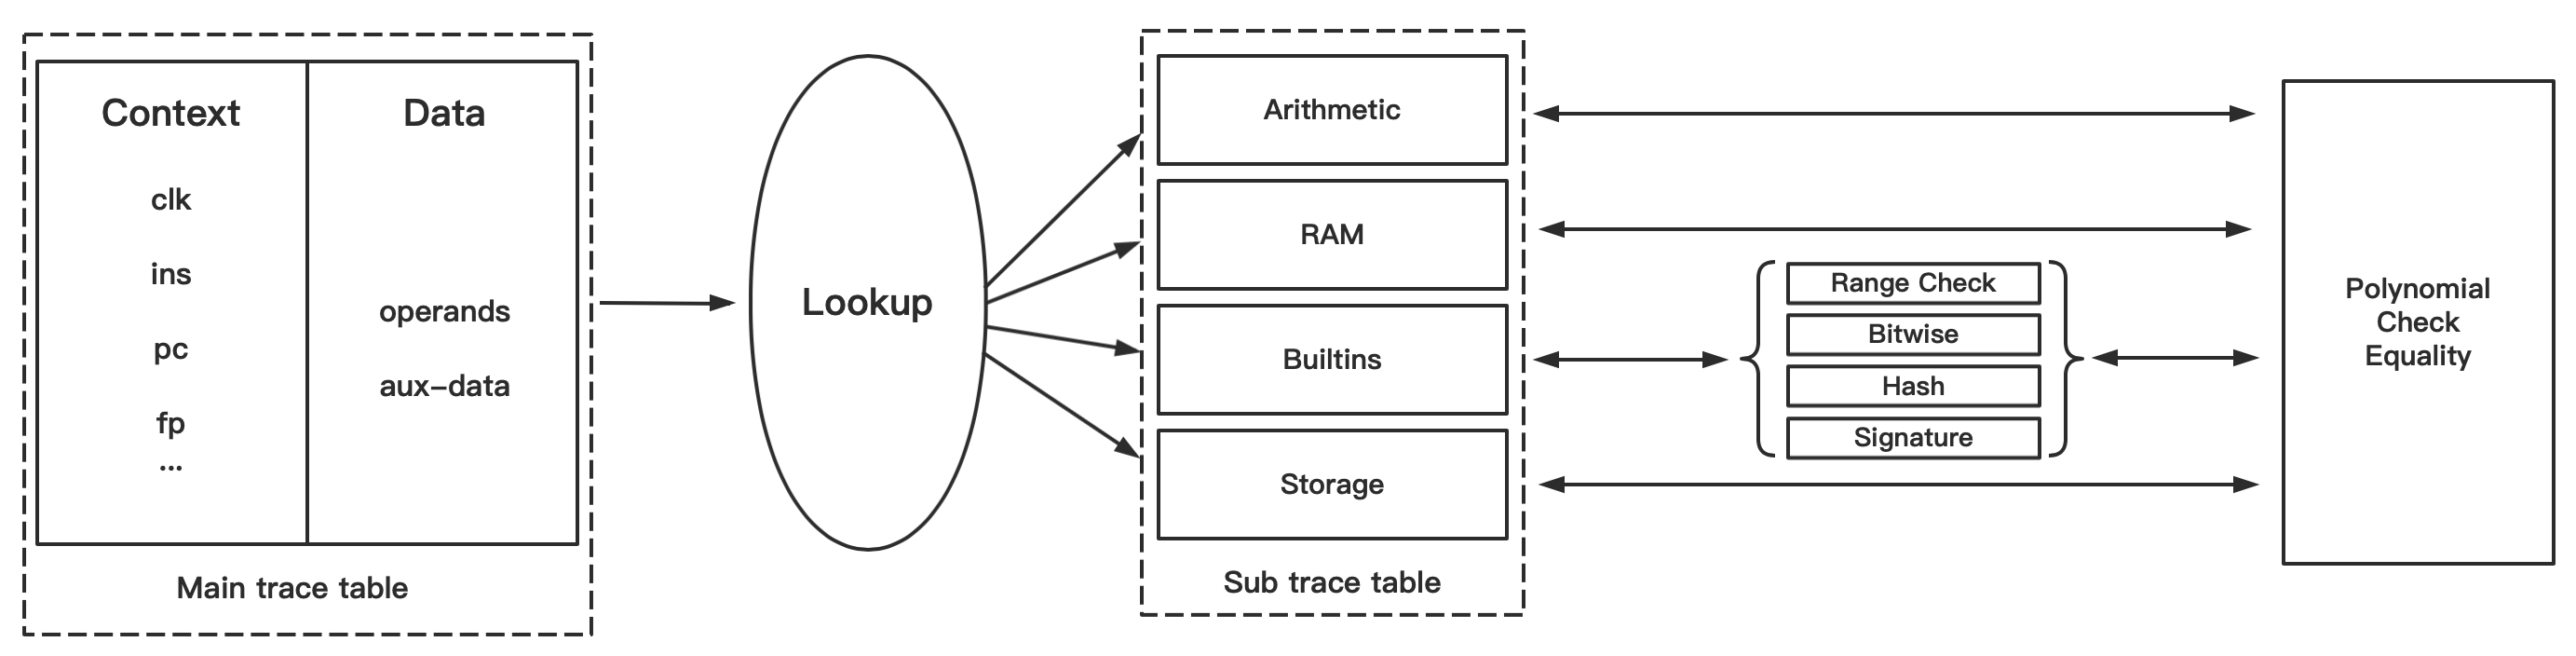
\includegraphics[width=\textwidth]{zkvm-architecture.png}
    \caption{Architecture of ZKVM}
    \label{fig:zkvm-architecture}
\end{figure}

The modular design approach allows for proofs among different modules to be executed in parallel, because the verification process is independent of each other, and the data correlation is only guaranteed by Permutation Argument and Lookup Argument, there are no data dependencies between each other. This is way more efficient than executing all the proofs in a single circuit, furthermore, multiple proofs corresponding to different sub-modules can be aggregated into a single proof, the idea of using recursive proofs can utilized to improve the system efficiency of proofs between different blocks.

These common technologies are all applied in OlaVM architecture.
